%%%%%%%%%%%%%%%
%
% $Autor: Wings $
% $Datum: 2020-01-29 07:55:27Z $
% $Pfad: General/IMUSoftware.tex
% $Version: 1785 $
%
%
%%%%%%%%%%%%%%%






\section{Bibliotheken}

Eine Bibliothek ist eine Sammlung von Quelltext und Funktionen, die es dem Anwender ermöglicht, zum Beispiel jegliche Sensoren bedienen zu können, ohne alle Rohdaten selbst zu verarbeiten. Für dieses Projekt wird die Bibliothek \PYTHON{Arduino\_LSM9DS1} des angesprochenen LSM9DS1 benötigt. In dieser Bibliothek sind die Funktionen enthalten, um die Bewegungen zu erfassen und in Winkel umzurechnen. Zusätzlich wird die Bibliothek \PYTHON{SSD1306Ascii}  zur Zeichendarstellung für das OLED-Display benötigt. \Mynote{citations for the libs}





\section{Beispiele auf dem Mikrocontroller}


\subsection{Testen des  Sensors LSM9DS1}

Das Beispiel \FILE{SimpleAccelerometer} wurde geladen und der Sensor gibt erfolgreich die Daten der Beschleunigung aus.

\begin{figure}[H]
    \centering
    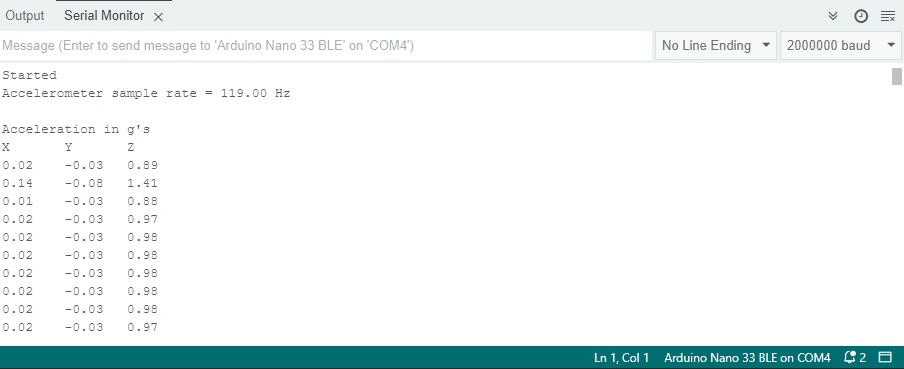
\includegraphics[width=\textwidth]{IMU/simpleaccelerometer}
    \caption{Output des Testprogramms}
\end{figure}



\section{Programmierung}

\subsection{Programmablaufplan}

\begin{figure}
    \centering
    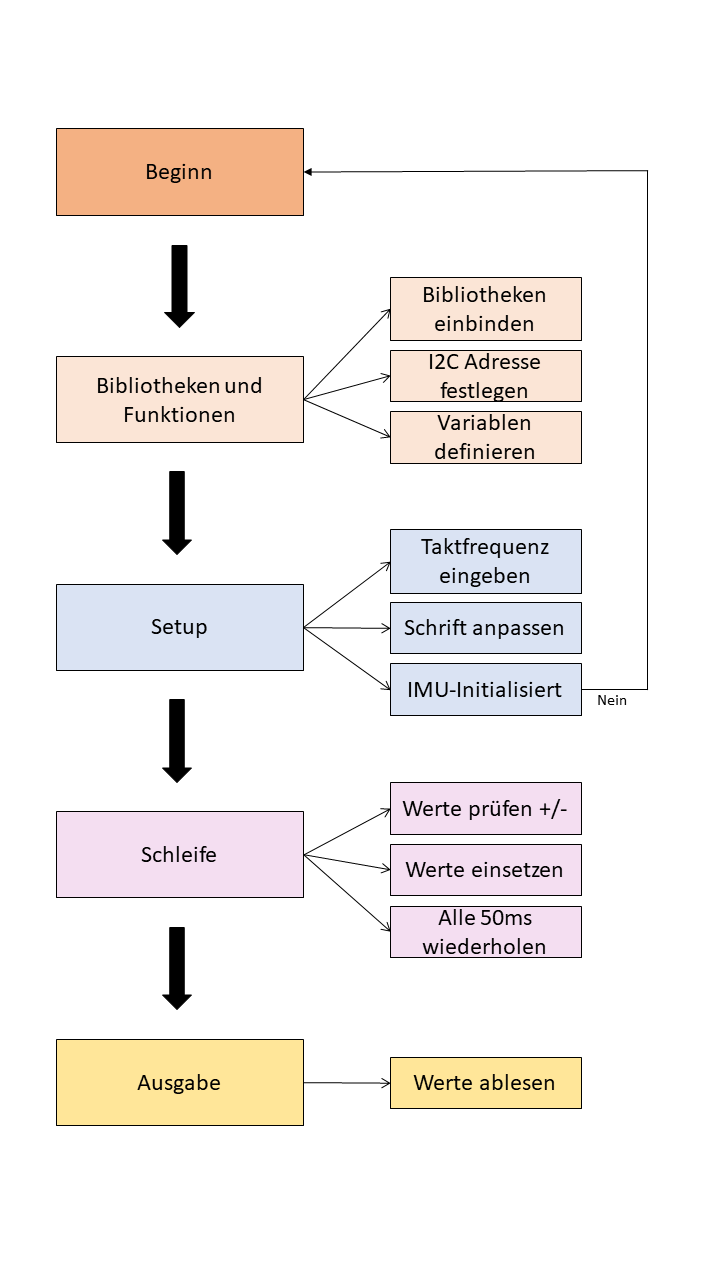
\includegraphics[width=\textwidth]{IMU/FlowChart}
    \caption{Der Programmablaufplan}
\end{figure}


\subsection{Programmcode und Dokumentation}

\begin{lstlisting}[language=Arduino]
#include <Arduino_LSM9DS1.h>
#include <Wire.h>
#include "SSD1306Ascii.h"
#include "SSD1306AsciiWire.h"
    
SSD1306AsciiWire oled;
    
#define I2C_ADDRESS 0x3C
#define RST_PIN -1
\end{lstlisting}



 Mit \PYTHON{\#include} werden die Bibliotheken eingebunden. In diesem Fall werden die Bibliotheken des  Sensors LSM9DS1 und die für das Display erforderliche \FILE{Wire.h} und \FILE{SSD1306Ascii.h} eingebunden. Über \PYTHON{\#define} werden die Adressen festgelegt, damit eine Kommunikation stattfinden kann. 



\begin{lstlisting}[language=Arduino]
float x, y, z;
int degreesX = 0;
int degreesY = 0;
String yPre, xPre;
\end{lstlisting}

Mit \PYTHON{float} (Gleitkommazahl / 4 Bytes) und \PYTHON{Int} (Ganzzahl / 4 Bytes) werden numerische Variablen definiert. In diesem Fall haben wir \PYTHON{degreesX} und \PYTHON{degreesY}, in denen wir unsere jeweiligen X- und Y-Werte für die Ausgabe erhalten. Diese werden zu Beginn auf 0 gesetzt. Die Strings (String=Zeichenkette) \PYTHON{yPre} und \PYTHON{xPre} werden hier implementiert um später die Vorzeichen der X- und Y-Achse zwischen zu speichern.


Nun beginnt das Setup. Hier handelt es sich um eine Funktion, die nur ein einziges Mal aufgerufen wird, sobald der Arduino startet. Da keine Rückgabewerte aus der Methode benötigt werden, wird die Funktionstype \PYTHON{void} verwendet. Die Funktion \PYTHON{Wire.setclock} definiert die Takt Frequenz für die I2C-Kommunikation. 

\begin{lstlisting}[language=Arduino]
void setup() 
{
  Wire.begin();
  Wire.setClock(400000L);
        
  #if RST_PIN >= 0
  oled.begin(&Adafruit128x64, I2C_ADDRESS, RST_PIN);
  #else   // RST_PIN >= 0
  oled.begin(&Adafruit128x64, I2C_ADDRESS);
  #endif  // RST_PIN >= 0      

  oled.setFont(TimesNewRoman16_bold);
  oled.clear();
  oled.println(" IMU Bereit");
        
  if (!IMU.begin()) 
  {
    oled.clear();
    oled.println("Failed to initialize IMU!");
    while (1);
  }
        
        
  xPre = "   ";
  yPre = "   ";
}
\end{lstlisting}

Die Funktion \PYTHON{oled.setFont} wird verwendet, um die Schriftart und Größe zu ändern. Bei der verwendeten Schriftart handelt es sich um \PYTHON{TimesNewRoman}. Um das Ablesen der Werte zu erleichtern ist die Schriftgröße 16 eingestellt. Der Befehl \PYTHON{oled.println} gibt nach dem Einschalten des Arduinos auf dem Display \PYTHON{''IMU Bereit''} aus. So soll dem Anwender mitgeteilt werden, dass die Messungen gestartet werden können. Falls die IMU nicht einsatzbereit sein sollte, wird über die \PYTHON{if}-Schleife \PYTHON{''Failed to initialize IMU!''} ausgegeben. Mit \PYTHON{xPre} und \PYTHON{yPre} werden aus optischen Gründen drei Leerzeichen definiert. So befinden sich auf der Anzeige die Messwerte geordnet übereinander.



\PYTHON{void loop}  bezeichnet eine Funktion, die jedes mal wenn sie am Ende ist wieder von vorne beginnt. In dieser Schleife werden die Werte, die der Sensor ausgibt, immer wieder aufgerufen und in die entsprechenden Ausgaben eingefügt. Dies sorgt für die Aktualisierung auf dem OLED-Display. 

In der ersten \PYTHON{if}-Abfrage wird abgefragt, ob der X-Wert größer ist als \PYTHON{0.1}. Wenn dies der Fall ist, merkt sich das Programm mit \PYTHON{xPre} das positive Vorzeichen. Die nächsten beiden \PYTHON{if}-Abfragen überprüfen, ob die entsprechenden Werte kleiner gleich 10 Grad sind (siehe Kap. 4.6). Wenn der Y-Wert kleiner gleich 10 Grad ist, gibt das Display die Ausgabe \PYTHON{''  X      0   Grad''} aus. Sobald der Wert größer als 10 Grad ist, beginnt \PYTHON{else} und gibt dem Display die Anweisungen \PYTHON{oled.print(''  X '');} für die Ausgabe des X-Wertes. Unmittelbar dahinter \PYTHON{oled.print(yPre);} für das gemerkte Vorzeichen von Y. Nun wird der vom Sensor gemessene Y-Wert für X eingesetzt \PYTHON{oled.print(degreesY);}. Zum Schluss wird mit \PYTHON{oled.print(''  Grad'');} Grad als Einheit hinter die Zeile gesetzt. Ausgaben wie \PYTHON{oled.print('' '');} beinhalten lediglich eine Leerzeile zur richtigen Ausrichtung der Werte untereinander. Die Funktion \PYTHON{map()} beschäftigt sich mit der Ganzzahlmathematik, dadurch werden selbst Brüche als ganze Zahlen weitergegeben. 

\bigskip
   
Info: Aufgrund des aufdruckten Koordinatensystems auf dem Gehäuse mussten die X- und Y-Werte getauscht werden, damit es für den Anwender bedienbar ist.


\begin{lstlisting}[language=Arduino]
void loop() 
{
  if (IMU.accelerationAvailable()) 
  {
    IMU.readAcceleration(x, y, z);
  }
  if (x > 0.1) 
  {
    x = 100 * x;
    degreesX = map(x, 0, 97, 0, 90);
            
    xPre = "+";
    oled.clear();
    oled.println();
            
    if (degreesY <= 10) 
    {
       oled.println("  X      0   Grad");
    } 
    else 
    {
      oled.print("  X ");
      oled.print(yPre);
      oled.print(" ");
      oled.print(degreesY);
      oled.print("  Grad");
      oled.println();
    }
    if (degreesX <= 10) 
    {
      oled.println("  Y      0   Grad");
    } 
    else 
    {
      oled.print("  Y + ");
      oled.print(degreesX);
      oled.print("  Grad");
      oled.println();
    }
  }      
\end{lstlisting}
    
Ab der Zeile \PYTHON{if (degreesX <= 10)} erfolgt der gleiche Prozess wie oben beschrieben für den entsprechenden Y-Wert.
        
Im Folgenden Programmauszug wird die Schleife für die anderen Richtungen wiederholt. Für die X-Werte unter \PYTHON{-0,1} wird mit \PYTHON{xPre = '' -'';} das Vorzeichen gemerkt und die Ausgaben wiederholen sich mit den entsprechenden Vorzeichen und Werten.
    
    \begin{lstlisting}[language=Arduino]
        if (x < -0.1) 
        {
            x = 100 * x;
            degreesX = map(x, 0, -100, 0, 90);
            
            xPre = " -";
            oled.clear();
            oled.println();
            
            if (degreesY <= 10) 
            {
                oled.println("  X      0   Grad");
            } 
            else 
            {
                oled.print("  X ");
                oled.print(yPre);
                oled.print(" ");
                oled.print(degreesY);
                oled.print("  Grad");
                oled.println();
            }
            
            if (degreesX <= 10) 
            {
                oled.println("  Y      0   Grad");
            } 
            else 
            {
                oled.print("  Y  - ");
                oled.print(degreesX);
                oled.print("  Grad");
                oled.println();
            }
        }
        
    \end{lstlisting}
    
    
Hier beginnt die Abfrage für die Y-Werte \PYTHON{if (y > 0.1)}. Sobald das Y positiv ist, wird sich mit \PYTHON{yPre = ''+'';} das Positive Vorzeichen gemerkt und die Schleife läuft wie vorher schon bei den X-Werten beschrieben.
    
    \begin{lstlisting}[language=Arduino]
        if (y > 0.1) 
        {
            y = 100 * y;
            degreesY = map(y, 0, 97, 0, 90);
            
            yPre = "+";
            oled.clear();
            oled.println();
            
            if (degreesY <= 10) 
            {
                oled.println("  X      0   Grad");
            } 
            else 
            {
                oled.print("  X + ");
                oled.print(degreesY);
                oled.print("  Grad");
                oled.println();
            }
            
            if (degreesX <= 10) 
            {
                oled.println("  Y      0   Grad");
            } 
            else 
            {
                oled.print("  Y ");
                oled.print(xPre);
                oled.print(" ");
                oled.print(degreesX);
                oled.print("  Grad");
                oled.println();
            }
        }
        if (y < -0.1) 
        {
            y = 100 * y;
            degreesY = map(y, 0, -100, 0, 90);
            
            yPre = " -";
            oled.clear();
            oled.println();
            
            if (degreesY <= 10) 
            {
                oled.println("  X      0   Grad");
            } 
            else 
            {
                oled.print("  X  - ");
                oled.print(degreesY);
                oled.print("  Grad");
                oled.println();
            }
            
            if (degreesX <= 10) 
            {
                oled.println("  Y      0   Grad");
            } 
            else 
            {
                oled.print("  Y ");
                oled.print(xPre);
                oled.print(" ");
                oled.print(degreesX);
                oled.print("  Grad");
                oled.println();
            }
        }
        delay(50);
    }
    
\end{lstlisting}

Hier endet die Schleife. Mit \PYTHON{delay(50)} wird sie alle 50 Millisekunden wiederholt. So wird die Aktualisierung des Displays realisiert. Der Winkelmesser funktioniert also in Echtzeit.\Mynote{Der Begriff Echtzeit ist nicht bekannt. Hier muss gemessen werden!}



\subsection{Definition Echtzeit}
\label{Echtzeit}
Echtzeit bedeutet, dass ein System auf ein Ereignis innerhalb eines vorgegebenen Zeitrahmens zuverlässig reagieren kann. Das System ist in der Lage, alle Daten innerhalb einer Zykluszeit einzulesen und ausgeben. \cite{Scholz:2005}


Sobald das Programm hochgeladen wurde, gibt es zwei wesentliche Ausgaben auf dem OLED-Display, die der Anwender nun sehen sollte.

\begin{figure}[H]
    \centering
    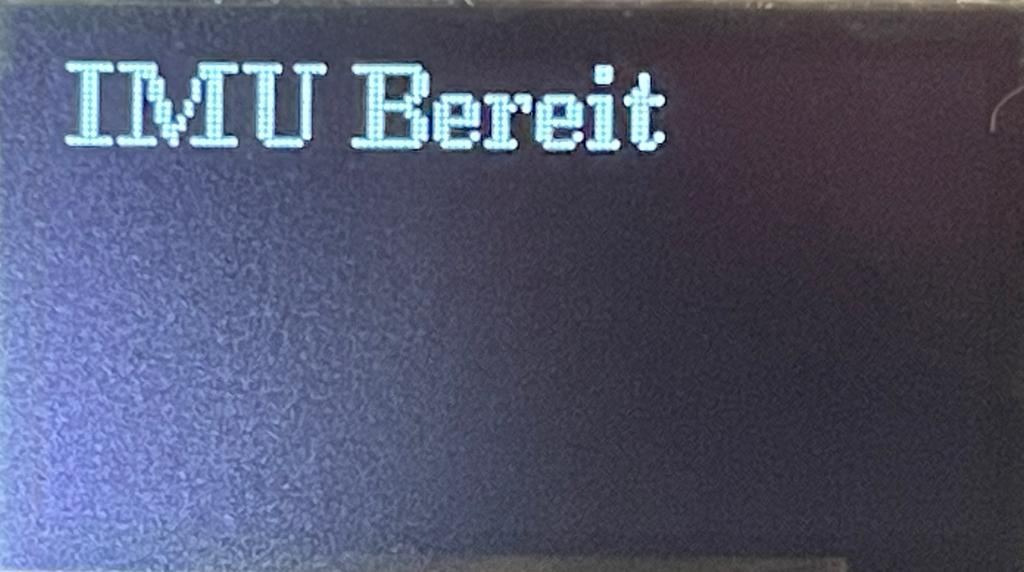
\includegraphics[width=0.8\textwidth]{OLED/OLEDBereit1}
    \caption{Anzeige des Arduino OLED Displays sobald der Arduino eingeschaltet ist}
\end{figure}

\begin{figure}[H]
    \centering
    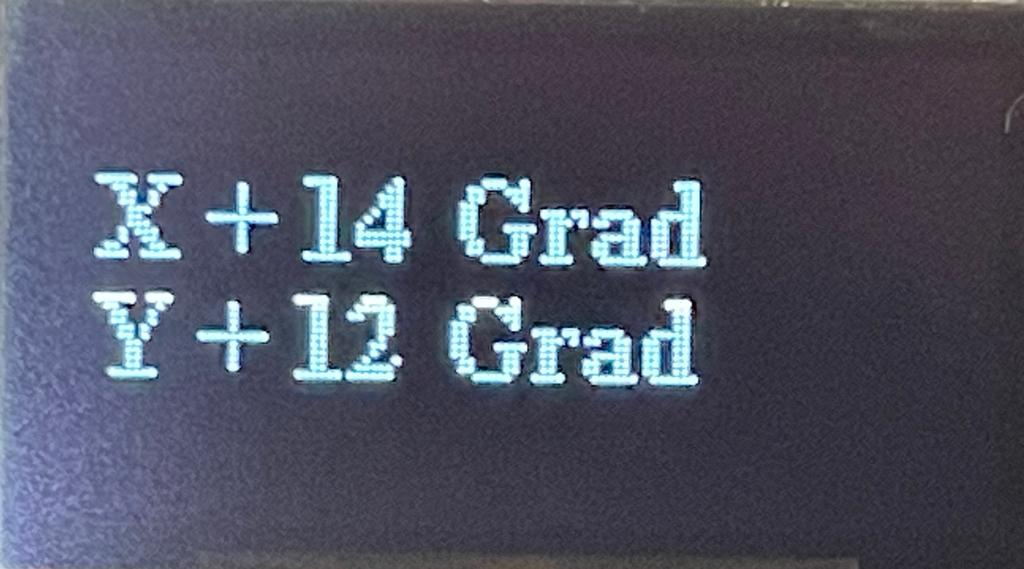
\includegraphics[width=0.8\textwidth]{OLED/OLEDBereit2}
    \caption{Ausgabe von Messdaten}
\end{figure}

\PYTHON{X+ 14 Grad, Y+ 12 Grad} ist eine Ausgabe von einer Beispielbewegung des Arduinos und zeigt dem Benutzer eine Mischung aus einem positiven X- und Y-Wert.




\section{Kalibrierung}

Es war weder möglich eine fertige Kalibrierungssoftware von GitHub oder einen von einer KI erstellten Quelltext zu nutzen, um das Gerät zu kalibrieren. Der Arduino selbst zeigt präzise Winkel bis 90 Grad an, war aber nicht in der Lage Winkel kleiner als 10 Grad auszugeben. Dementsprechend wurde die if-Abfrage eingebaut, um Winkel die kleiner gleich 10 Grad sind auf dem Display als 0 Grad ausgegeben werden.



\section{Probleme}

Aufgrund mehrerer Fehler mit der seriellen Schnittstelle wurde zu Beginn angenommen, dass der Arduino einen Defekt hat. Nach weiteren Nachforschungen stellten wir allerdings fest, dass der Arduino sich ganz einfach zurücksetzen lässt. Mithilfe des kleinen Knopfs auf dem Arduino-Board, startet dieser in den Bootloader und lässt sich dann mit einer manuellen Änderung des COM-Ports wieder bespielen.

\begin{figure}[H]
    \centering
    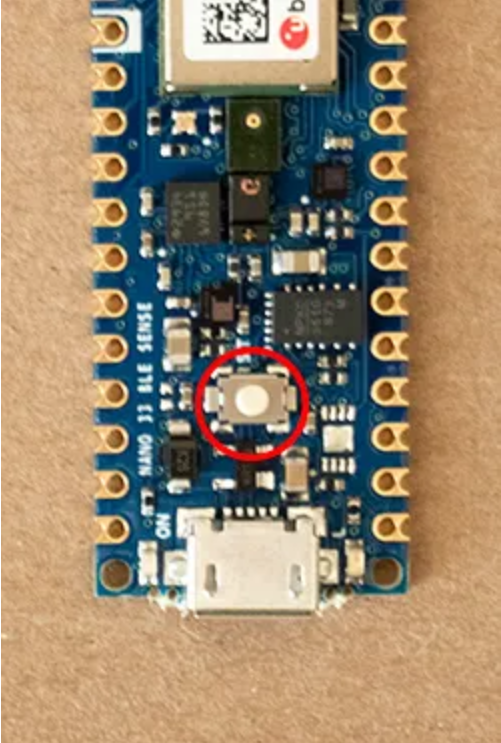
\includegraphics[width=0.8\textwidth]{Nano33BLESense/reset}
    \caption{Der Reset Button des Arduino}
\end{figure}





